\documentclass[pdftex,12pt,a4paper]{article}

\usepackage[pdftex]{graphicx}
\usepackage{paralist}
\usepackage{mathtools}
\usepackage{hyperref}
\usepackage[xindy]{glossaries}

\newcommand{\HRule}{\rule{\linewidth}{0.5mm}}

\newglossaryentry{OpenGL}
{
  name=OpenGL,
  description={stands for Open Graphics Library and is a cross-language, multi-platform application programming interface (API) for rendering 2D and 3D computer graphics\footnote{http://en.wikipedia.org/wiki/OpenGL}}
}

\newglossaryentry{OpenGL ES}
{
  name=OpenGL ES,
  description={OpenGL for Embedded Systems (OpenGL ES) is a subset of the OpenGL computer graphics rendering application programming interface (API) for rendering 2D and 3D computer graphics such as those used by video games, typically hardware-accelerated using a graphics processing unit (GPU)\footnote{http://en.wikipedia.org/wiki/OpenGL\_ES}}
}

\newglossaryentry{Versor (libvsr)}
{
  name=Versor (libvsr),
  description={is a C++ Library for Geometric Algebra with built-in draw routines\footnote{https://github.com/wolftype/vsr2.0/}}
}

\newglossaryentry{geometric algebra}
{
  name=Geometric Algebra (GA),
  description={is the Clifford algebra of a vector space over the field of real numbers endowed with a quadratic form \footnote{http://en.wikipedia.org/wiki/Geometric\_algebra}}
}

\newglossaryentry{GLV}
{
  name=GLV,
  description={is a GUI building toolkit written in C++ for Linux, OSX, and Win32\footnote{https://github.com/AlloSphere-Research-Group/GLV}}
}

\newglossaryentry{GFX}
{
  name=GFX,
  description={is a generic graphics library (using OpenGL and OpenGL ES 2.0)\footnote{https://github.com/wolftype/gfx}}
}

\newglossaryentry{bivector}
{
  name=Bivector,
  description={is a quantity in exterior algebra or geometric algebra that extends the idea of scalars and vectors\footnote{http://en.wikipedia.org/wiki/Bivector}}
}

\newglossaryentry{GLUT}
{
  name=GLUT,
  description={stands for OpenGL Utility Toolkit and is a library of utilities for OpenGL programs, which primarily perform system-level I/O with the host operating system\footnote{http://en.wikipedia.org/wiki/OpenGL\_Utility\_Toolkit}}
}

\newglossaryentry{cube mapping}
{
  name=Cube mapping,
  description={is a method of environment mapping that uses the six faces of a cube as the map shape within the field of computer graphics\footnote{http://en.wikipedia.org/wiki/Cube\_mapping}}
}
\makeglossaries


\begin{document}
%deckblatt start
\thispagestyle{empty}
\begin{center}
\Large{Berne University of Applied Sciences (BFH)}\\
\end{center}
 
 
\begin{center}
\Large{Department Engineering and information technology}
\end{center}
\begin{verbatim}
\end{verbatim}
\begin{center}
\textbf{\LARGE{BZG1310 -  Object-oriented geometry}}
\end{center}
\begin{verbatim}
 
 
\end{verbatim}
\begin{center}
\textbf{Documentation Project 1}
\end{center}
\begin{verbatim} 
\end{verbatim}
 
\begin{flushleft}
\begin{tabular}{lll}
\textbf{Subject:} & & Spinning cube with spheres on its edges --\\
& & Classical approach using OpenGL and GLSL\\
& & \\
& & \\
& & \\
\textbf{Student:} & & Sven Osterwalder (ostes2@bfh.ch)\\
& & \\
& & \\
\textbf{Date:} & & {\today}\\
& & \\
& & \\
\textbf{Professor:} & & M. Stampfli
\end{tabular}
\end{flushleft}

\newpage

\section{Management summary}

This dissertation is part of a project in the context of the subject \textit{BZG1310: Object-oriented geometry} at Bern University of Applied Sciences.
\\
\\
The goal of this project is the implementation of a rotating cube which has a sphere on each edge using methods of \gls{geometric algebra} within the field of computer graphics.
\\
\\
The goal could be reached and the task was implemented using C++ and \gls{Versor (libvsr)}.\\
\\
\begin{figure}[htbp]
\centering \rotatebox{0}{\scalebox{0.2}[0.2]{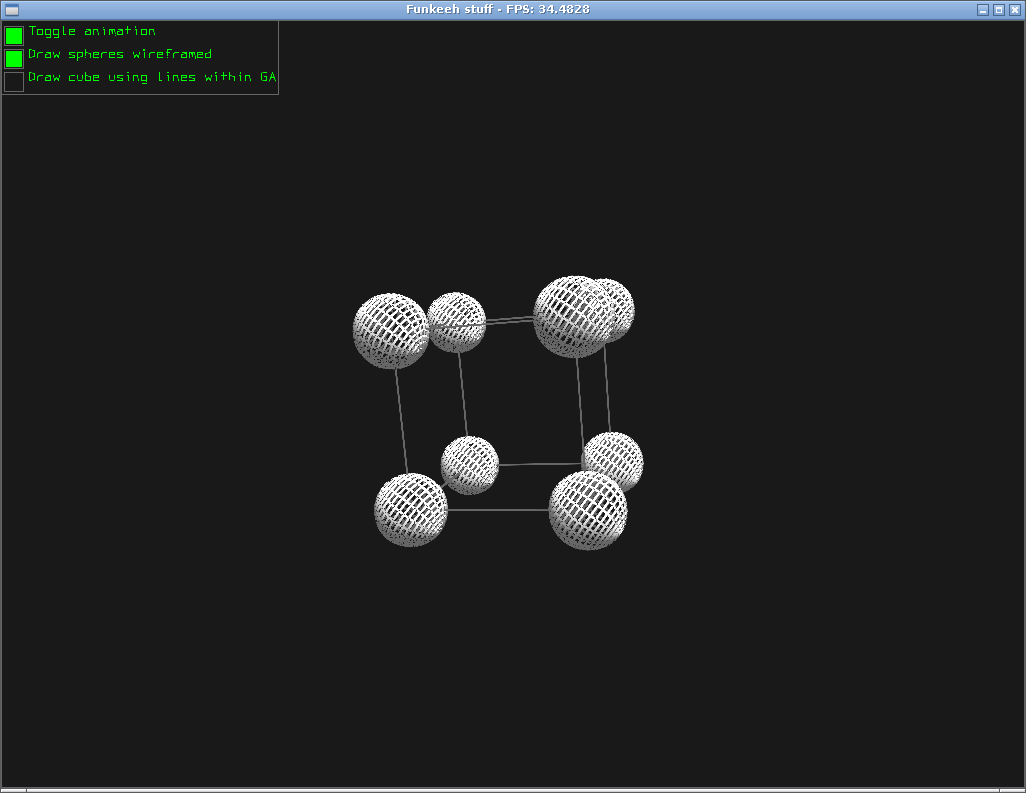
\includegraphics{screenshot.png}}}
\caption{Screenshot of the running application \label{fig:screenshot}}
\end{figure}

\section{Implementation}

The implementation was done using C++ and the Versor library.

\subsection{Versor library}

To cover the main tasks such as providing minimal application logic or handling input the Versor library was used as it provides drawing routines using an external library called \gls{GFX} based upon \gls{OpenGL} as well as a graphical user interface using another external library called \gls{GLV}.
\newpage

\subsection{Geometric operations}

As the geometric operations are the main aspect of the course BZG1310, this section shows how this aspect was realized within the application.\\

\subsubsection{Implementation of the cube}
For drawing the cube two methods were implemented:
\begin{compactitem}
	\item One using the \textit{NCube} class built-in in Versor
	\item One using lines
\end{compactitem}
\vspace*{2mm}
\noindent\hspace*{0mm}The method using the \textit{NCube} class has the advantage that the lines are finite, therefore they begin and end at certain, defined points in space.\\
When using lines there remains the problem that the lines do not end, given the implementation in Versor:\vspace*{5mm}\\
\noindent\hspace*{10mm}\vspace*{5mm} $ a \wedge b \wedge Inf(1) $

\subsubsection{Implementation of the spheres}
The spheres were implemented using the \textit{sphere} class from Versor:\vspace*{5mm}\\
\noindent\hspace*{10mm}\vspace*{5mm} $ Ro::sphere(PositionOfSphere, SphereRadius); $

\subsubsection{Rotations}
Versor provides two methods to implement rotations:\\
\begin{compactitem}
	\item Using the \textit{rot()} method on objects
	\item Using generators
\end{compactitem}
\vspace*{2mm}
\noindent\hspace*{0mm}In this project only the first method was used to apply rotations. The rotations were realized using a \gls{bivector} whose coordinates are based on a timer\footnote{which is the current time in milliseconds minus the time when the application was started in milliseconds} object:\vspace*{5mm}\\
\noindent\hspace*{10mm}\vspace*{5mm} $ bivRotation = Biv(sinf(fTime * 0.001f), 0, cosf(fTime * 0.001f)); $\\
\noindent\hspace*{0mm}This bivector is then applied to each vector which defines the coordinates of a sphere respectively the edges of the cube:\vspace*{5mm}\\
\noindent\hspace*{10mm}\vspace*{5mm} $ Ro::sphere(Vec(-0.5, 0.5, -0.5).rot(bivRotation), fSphereRadius); $\\
\noindent\hspace*{10mm}\vspace*{5mm} $  Fl::line(topLeftBack.rot(bivRotation), topRightBack.rot(bivRotation)); $\\
\noindent\hspace*{10mm}$ gfx::Glyph::Line(\\
	\noindent\hspace*{15mm}vecCube[edge.a].rot(bivRotation),\\
	\noindent\hspace*{15mm}vecCube[edge.b].rot(bivRotation)\\
\noindent\hspace*{10mm}); $\\
\\
\noindent\hspace*{0mm}To provide a rotation for the spheres along their own axis resp. axes quite a lot of effort was made to realize this with operations within geometric algebra - sadly without any good results.\\
Versor always seems to need an offset for applying rotations, therefore a rotation with the basis $ Vec(0, 0, 0) $ will not work. Neither when a translation is applied before or afterwards.\\
To achieve a rotation of the spheres along their own axes, a similar approach as used in the \textit{GFX} library was used: Direct usage of the OpenGL command \textit{glRotatef}.\\
This is not very sophisticated nor are operations from geometric algebra used but there seems currently no other way to achieve the task.

\section{Conclusion}
The \textit{Versor} library seems to provide a quick way for making use of geometric algebra to realize graphical applications.\\
Nevertheless I personally think that the implementation or maybe even the subject is in a rather early stage for being a replacement for the conventional and yet used methods.\\
\\
The library seems not to be up-to-date concerning the rendering as it makes use of conventional render methods such als \textit{glVertex3f} and even \gls{GLUT}.\\
Furthermore I think it would rather be hard or even impossible (at least at the moment) to implement things as for example \gls{cube mapping}.\\
\\
At the end all gets realized using conventional methods within OpenGL. In my humble opinion it will provide an advantage to the currently used methods if the hardware supports it as well.\\
All in all it was an interesting experience on a not so explored subject.

\printglossary[numberedsection]

\end{document}